
\documentclass[12pt]{article}
\pagestyle{empty} \topmargin -0.5in \textheight 9in \textwidth 6.5in
\oddsidemargin -0in
\usepackage{amssymb}
\usepackage{amsmath}
\usepackage[normalem]{ulem}
\usepackage{enumerate}
\usepackage{xcolor}
\usepackage{graphicx}

\DeclareMathOperator{\tr}{tr}

\newcommand{\vect}[1]{\mathbf{#1}}
\newcommand{\mcE}{\mathcal{E}}

\begin{document}

\begin{flushleft}

\textbf{Department of Applied Mathematics and Statistics}

\textbf{COLORADO SCHOOL OF MINES}\\


MATH $455$: Partial Differential Equations
\end{flushleft}

\vspace{0.1in}

\begin{center}
{\bf Assignment \#3 - Wave Equation} \\
Due Tuesday, October 6, 2026 \\
\end{center}

\vspace{0.1in}

\noindent $\textbf{1}$. (15 points) Define the functions
$$f(x) =
\begin{cases}
	x, & \mathrm{if} \ 0 \leq x \leq 1 \\ 
	1, & \mathrm{if} \ 1 < x < 5 \\ 
	6-x, & \mathrm{if} \ 5 \leq x \leq 6 \\ 
	0, & \mathrm{else},
\end{cases}$$
$$g(x) =
\begin{cases}
	1, & \mathrm{if} \ |x| < 1 \\ 
	0, & \mathrm{else},
\end{cases}$$
and consider solutions of the wave equation
\begin{equation}
\label{WE}
\tag{WE}
 \frac{\partial^2 u}{\partial t^2} -c^2 \frac{\partial^2 u}{\partial x^2} = 0.
\end{equation}
\begin{enumerate}[(a)]
\item Graph $f(x)$ and $g(x)$ by hand. \\ \\
\textcolor{blue}{\textbf{Solution} — 
\begin{figure}[h]
    \centering 
    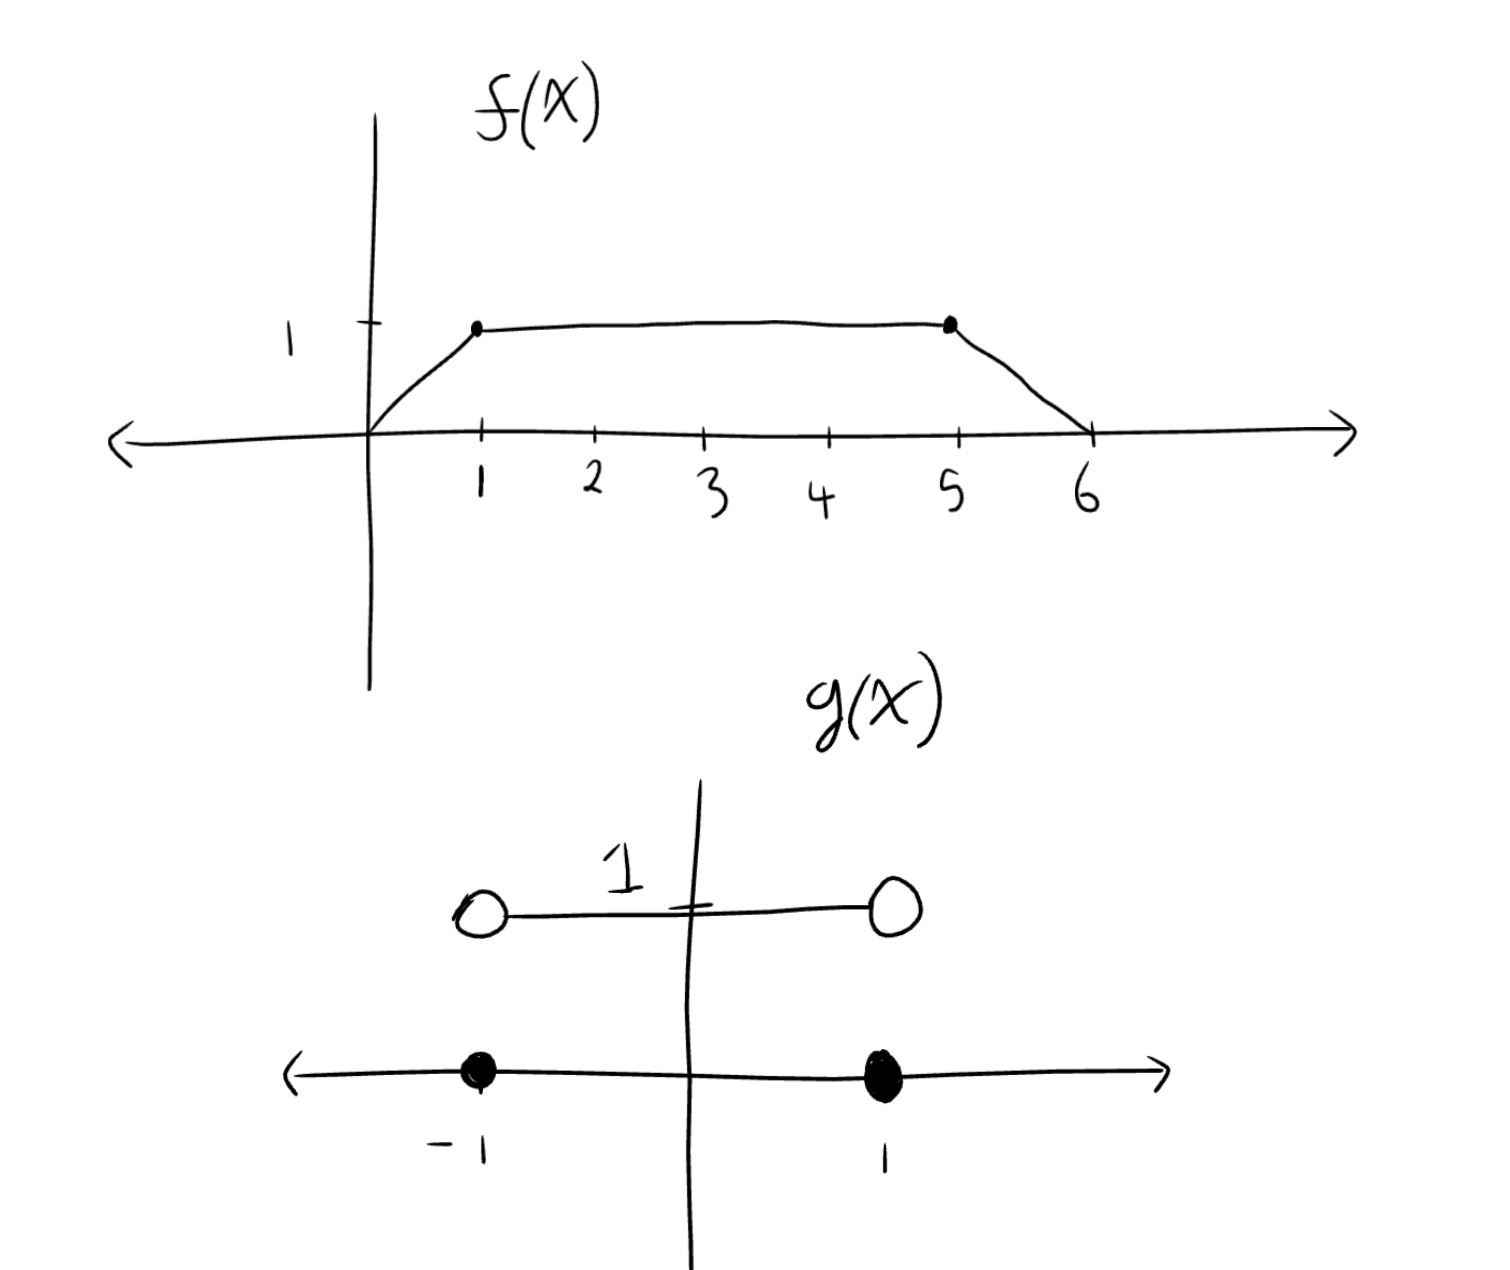
\includegraphics[width=0.5\textwidth]{Q1}
\end{figure} \\}

\item Find the solution of \eqref{WE} for $x \in \mathbb{R}, t > 0$ with 
$$u(0,x) = f(x) \quad \mathrm{and} \quad \frac{\partial u}{\partial t}(0,x) = 0$$
for $x \in \mathbb{R}$. In particular, write the solution in terms of the $f(x)$ function. Then, graph by hand $u(\frac{1}{c},x)$, $u(\frac{2}{c},x)$, and $u(\frac{3}{c},x)$ using different axes. \\ \\
\textcolor{blue}{\textbf{Solution} — To find the general solution of (WE), apply the substitution
\begin{align*}
& r(x,t) = x - ct \\
& s(x,t) = x + ct
\end{align*}
Assume $u(x,t) = U(r,s)$ is a solution and substitute (we first calculate the needed derivatives of $u$):
\begin{align*}
\frac{\partial u}{\partial x} &= \frac{\partial U}{\partial r} \frac{\partial r}{\partial x} + \frac{\partial U}{\partial s} \frac{\partial s}{\partial x} \\ \\
&= \frac{\partial U}{\partial r} +  \frac{\partial U}{\partial s}
\end{align*}
And 
\begin{align*}
\frac{\partial^2 u}{\partial x^2} &= \frac{\partial}{\partial x} \left( \frac{\partial U}{\partial r} +  \frac{\partial U}{\partial s}  \right) \\
\end{align*}
To simplify further, note that $\frac{\partial U}{\partial r}$ is some function of $r$ and $s$, say $\phi_1(r,s)$, and $\frac{\partial U}{\partial s}$ is also some function of $r$ and $s$, say $\phi_2(r,s)$:
\begin{align*}
&= \frac{\partial}{\partial x} \left( \phi_1(r,s) +  \phi_2(r,s)  \right) \\ \\
&= \frac{\partial \phi_1}{\partial r} \frac{\partial r}{\partial x} + \frac{\partial \phi_1}{\partial s} \frac{\partial s}{\partial x} + \frac{\partial \phi_2}{\partial r} \frac{\partial r}{\partial x} + \frac{\partial \phi_2}{\partial s} \\ \\
&= \frac{\partial \phi_1}{\partial r} + \frac{\partial \phi_1}{\partial s} + \frac{\partial \phi_2}{\partial r} + \frac{\partial \phi_2}{\partial s} \\ \\
&= \frac{\partial}{\partial r} \left( \frac{\partial U}{\partial r} \right) + \frac{\partial}{\partial s} \left( \frac{\partial U}{\partial r} \right) + \frac{\partial}{\partial r} \left( \frac{\partial U}{\partial s} \right) + \frac{\partial}{\partial s} \left( \frac{\partial U}{\partial s} \right) \\ \\
&= \frac{\partial^2 U}{\partial r^2} + \frac{\partial^2 U}{\partial s \partial r} + \frac{\partial^2 U}{\partial r \partial s} + \frac{\partial^2 U}{\partial s^2} 
\end{align*}
Let us assume that $U(r,s)$ is smooth and well-behaved enough for the cross-derivatives to be equal. Then
\begin{align*}
\frac{\partial^2 u}{\partial x^2} &= \frac{\partial^2 U}{\partial r^2} + 2 \left( \frac{\partial^2 U}{\partial r \partial s} \right) + \frac{\partial^2 U}{\partial s^2} 
\end{align*}
}


\item Find the solution of \eqref{WE} for $x \in \mathbb{R}, t > 0$ with 
$$u(0,x) = 0 \quad \mathrm{and} \quad \frac{\partial u}{\partial t}(0,x) = g(x)$$
for $x \in \mathbb{R}$. In particular, write the solution in terms of the $g(x)$ function. Then, graph by hand $u(\frac{1}{c},x)$, $u(\frac{2}{c},x)$, and $u(\frac{3}{c},x)$ using different axes. \\ \\
\textcolor{blue}{\textbf{Solution} — }

\end{enumerate}

\vspace{0.2in}

\noindent $\textbf{2}$. (12 points) Let $f, g \in \mathrm{PC}^1[0,L]$ be given continuous functions. Find the solution of \eqref{WE}
for $0 < x < L$ and $t > 0$
with the boundary conditions
$$\frac{\partial u}{\partial x}(t,0) = \frac{\partial u}{\partial x}(t,L) =0 , \qquad t > 0$$
and the initial conditions for $0 < x < L$
$$ u(0,x) = f(x), \quad \frac{\partial u}{\partial t}(0,x) = g(x).$$ \\ \\
\textcolor{blue}{\textbf{Solution} — }

\vspace{0.2in}

\noindent $\textbf{3}$. (15 points) Assume $u(t,x)$ satisfies \eqref{WE} for $0 < x < L$ and $t > 0$
and define
$$\mcE(t) = \frac{1}{2} \int_0^L \left | \frac{\partial u}{\partial t}(t,x) \right |^2 dx + \frac{1}{2}c^2 \int_0^L \left |  \frac{\partial u}{\partial x}(t,x)  \right |^2  dx$$
to be the associated total energy, where the first term in $\mcE(t)$ represents the kinetic energy and the second represents the potential energy.
\begin{enumerate}[(a)]
\item Use \textbf{integration by parts} to show that the total energy satisfies
$$\mcE'(t) = c^2  \frac{\partial u}{\partial t}(t,x)  \frac{\partial u}{\partial x}(t,x)  \biggr \vert_{x=0}^{x=L}.$$ \\ \\
\textcolor{blue}{\textbf{Solution} — }

\vspace{0.01in}

\item Show that the energy is conserved, meaning $\mcE(t) = \mcE(0)$ for all $t \geq 0$, for the zero Neumann boundary condition, namely assume that for $t \geq 0$
$$ \frac{\partial u}{\partial x} (t,0) = 0 \qquad \mathrm{and}  \qquad \frac{\partial u}{\partial x} (t,L) = 0.$$ \\ \\ 
\textcolor{blue}{\textbf{Solution} — }

\item Show that the energy is conserved for any Dirichlet boundary conditions, namely for given $A,B \in \mathbb{R}$ assume that for $t \geq 0$
$$u(t,0) = A \qquad \mathrm{and} \qquad u(t,L) = B.$$ \\ \\
\textcolor{blue}{\textbf{Solution} — }


\item Show that the potential energy and kinetic energy are equal for a traveling wave solution
$$u(t,x) = v(x-ct)$$
where $v$ is a sufficiently smooth function. \\ \\
\textcolor{blue}{\textbf{Solution} — }
\end{enumerate}

\vspace{0.2in}


\noindent $\textbf{4}$. (8 points) Maxwell's equations for electric $E(t,x)$ and magnetic $B(t,x)$ fields in a vacuum are
$$
\left \{
\begin{gathered}
\frac{\partial B}{\partial t} + \nabla \times E = 0\\
\mu_0\epsilon_0\frac{\partial E}{\partial t} - \nabla \times B = 0\\
\nabla \cdot E =\nabla \cdot B = 0
\end{gathered} 
\right.
$$
where $\mu_0> 0$ is the permeability of free space and
$\epsilon_0>0$ is the permittivity of free space.
Using the ``curl-curl'' identity
$$ \nabla \times \left (\nabla \times \phi \right ) = \nabla \left ( \nabla \cdot \phi \right ) - \Delta \phi$$
for any $\phi(x)$,
show that both $E$ and $B$ satisfy the (vector) wave equation 
$$\frac{\partial^2 u}{\partial t^2} -c^2 \Delta u = 0$$
and determine the associated speed of propagation $c$.
Here, $\Delta \phi = \nabla \cdot (\nabla \phi)$ is the Laplacian of $\phi$, which represents a generalization of the second derivative in higher dimensions. \\ \\
\textcolor{blue}{\textbf{Solution} — }


\end{document}
